% filepath: d:\GitHub\DoutoradoCefet\AlgoritmoEstruturaDados\Trabalho\Relatorio\relatorio.tex
\documentclass[12pt]{article}
\usepackage[brazil]{babel}
\usepackage[utf8]{inputenc}
\usepackage{graphicx}
\usepackage{amsmath}
\usepackage{geometry}
\usepackage{multirow}
\usepackage{float}
\usepackage{setspace}
\usepackage{titlesec}
\usepackage{indentfirst}
\geometry{a4paper, left=3cm, right=2cm, top=3cm, bottom=2cm}

\setlength{\parindent}{1.5cm}
\setlength{\parskip}{0.2cm}
\onehalfspacing

\titlespacing*{\section}{0pt}{*4}{*2}
\titlespacing*{\subsection}{0pt}{*2}{*1.5}
\titlespacing*{\subsubsection}{0pt}{*1.5}{*1}

\begin{document}

% Capa (modelo ABNT simplificado)
\begin{titlepage}
\begin{center}
    \large
    \textbf{CENTRO FEDERAL DE EDUCAÇÃO TECNOLÓGICA DE MINAS GERAIS}\\
    \textbf{DOUTORADO EM MODELAGEM MATEMÁTICA COMPUTACIONAL}\\
    \textbf{ALGORITMOS E ESTRUTURAS DE DADOS}\\
    \vspace{4cm}
    \textbf{COMPARAÇÃO DOS MÉTODOS DE ORDENAÇÃO QUICKSORT E HEAPSORT}\\
    \vspace{4cm}
    Leonardo Vieira Guimarães\\
    \vfill
    Belo Horizonte\\
    \the\year
\end{center}
\thispagestyle{empty}
\end{titlepage}

% Removido o \newpage após a capa para que o resumo fique na página seguinte sem número

\newpage
\pagenumbering{arabic}

\tableofcontents
\newpage

\section{Introdução}
A ordenação de dados é uma das tarefas fundamentais em Ciência da Computação, sendo essencial para otimizar buscas, análises e diversas operações em estruturas de dados. Entre os algoritmos clássicos de ordenação, destacam-se o Quicksort e o Heapsort, ambos amplamente utilizados devido à sua eficiência e aplicabilidade em diferentes contextos.

O objetivo deste trabalho é realizar uma análise comparativa entre os algoritmos Quicksort (utilizando sempre o primeiro elemento como pivô) e Heapsort, com foco no número de comparações realizadas durante a ordenação de vetores em diferentes cenários: vetores já ordenados em ordem crescente (melhor caso), vetores ordenados em ordem decrescente (pior caso) e vetores com elementos aleatórios (caso médio). A partir dessa análise, busca-se compreender o impacto da escolha do algoritmo e das características da entrada no desempenho observado, destacando vantagens, limitações e situações em que cada método se mostra mais eficiente.

\section{Desenvolvimento}

Para atender ao objetivo do trabalho, foram seguidos os seguintes passos:

\begin{enumerate}
    \item \textbf{Implementação dos métodos de ordenação:}
    \begin{itemize}
        \item \textbf{Quicksort:} pivô sempre o primeiro elemento do vetor.
        \item \textbf{Heapsort:} construção do heap máximo e ordenação por remoção sucessiva do maior elemento.
    \end{itemize}
    \item \textbf{Testes realizados para cada método:}
    \begin{enumerate}
        \item[a)] Gerar vetores de $n$ elementos \textbf{ordenados em ordem crescente}, com $n$ variando de 1000 até 10.000, com intervalo de 1000. Ordenar esses vetores com ambos os métodos e computar o número de comparações realizadas.
        \item[b)] Gerar vetores de $n$ elementos \textbf{ordenados em ordem decrescente}, com $n$ variando de 1000 até 10.000, com intervalo de 1000. Ordenar esses vetores com ambos os métodos e computar o número de comparações realizadas.
        \item[c)] Gerar vetores de $n$ elementos \textbf{aleatórios}, com $n$ variando de 1000 até 10.000, com intervalo de 1000. Ordenar esses vetores com ambos os métodos e computar o número de comparações realizadas.
        \item[d)] Fazer um único gráfico de $n$ versus número de comparações, levando em consideração todos os testes realizados.
    \end{enumerate}
     \item \textbf{Análise dos comportamentos dos gráficos gerados}
\end{enumerate}



A Tabela~\ref{tab:complexidade} apresenta as fórmulas de recorrência e as ordens de complexidade assintótica dos algoritmos Quicksort e Heapsort para os diferentes cenários (melhor caso, caso médio e pior caso) analisados neste trabalho, nesta tabela podemos observar que ambos os algoritmos possuem complexidade $O(n \log n)$ no melhor caso e no caso médio, mas o Quicksort apresenta complexidade $O(n^2)$ no pior caso, enquanto o Heapsort mantém $O(n \log n)$.

\begin{table}[h!]
\centering
\begin{tabular}{|l|l|l|l|l|}
\hline
\multirow{2}{*}{\textbf{Caso}} & \multicolumn{2}{|c|}{\textbf{Quicksort}} & \multicolumn{2}{|c|}{\textbf{Heapsort}} \\
\cline{2-5}
 & $\textbf{T(n)}$ & $\textbf{O}$ & $\textbf{T(n)}$ & $\textbf{O}$ \\
\hline
Melhor & $2T(\frac{n}{2}) + cn$ & $O(n \log n)$ & $O(n) + nO(\log n)$ & $O(n \log n)$ \\
\hline
Médio  & $2T(\frac{n}{2}) + cn$ & $O(n \log n)$ & $O(n) + nO(\log n)$ & $O(n \log n)$ \\
\hline
Pior   & $T(n-1) + cn$ & $O(n^2)$ & $O(n) + nO(\log n)$ & $O(n \log n)$ \\
\hline
\end{tabular}
\caption{Resumo das complexidades de Quicksort e Heapsort.}
\label{tab:complexidade}
\end{table}


\subsection{Experimentos e Plotagem dos Resultados}

Para a realização dos experimentos, os algoritmos Quicksort e Heapsort foram implementados em Python, seguindo rigorosamente as especificações do enunciado. Os testes seguiram os seguintes passos:

\begin{enumerate}
    \item Para cada valor de $n$ no intervalo de 1000 a 10.000 (com incremento de 1000), foram gerados três tipos de vetores: ordenados em ordem crescente, ordenados em ordem decrescente e aleatórios.
    \item Cada vetor foi ordenado utilizando ambos os algoritmos, e o número de comparações realizadas foi registrado.
    \item Os resultados foram utilizados para gerar gráficos que relacionam o tamanho do vetor ($n$) ao número de comparações realizadas.
\end{enumerate}

\subsubsection{Resultados para Vetores Ordenados em Ordem Crescente (Melhor Caso)}

Foram gerados vetores ordenados em ordem crescente, variando de 1000 a 10.000 elementos. Cada vetor foi ordenado utilizando Quicksort e Heapsort, e o número de comparações foi registrado.

O gráfico (Figura~\ref{fig:crescente}) mostra o número de comparações realizadas por cada algoritmo para vetores ordenados em ordem crescente:

\begin{figure}[H]
    \centering
    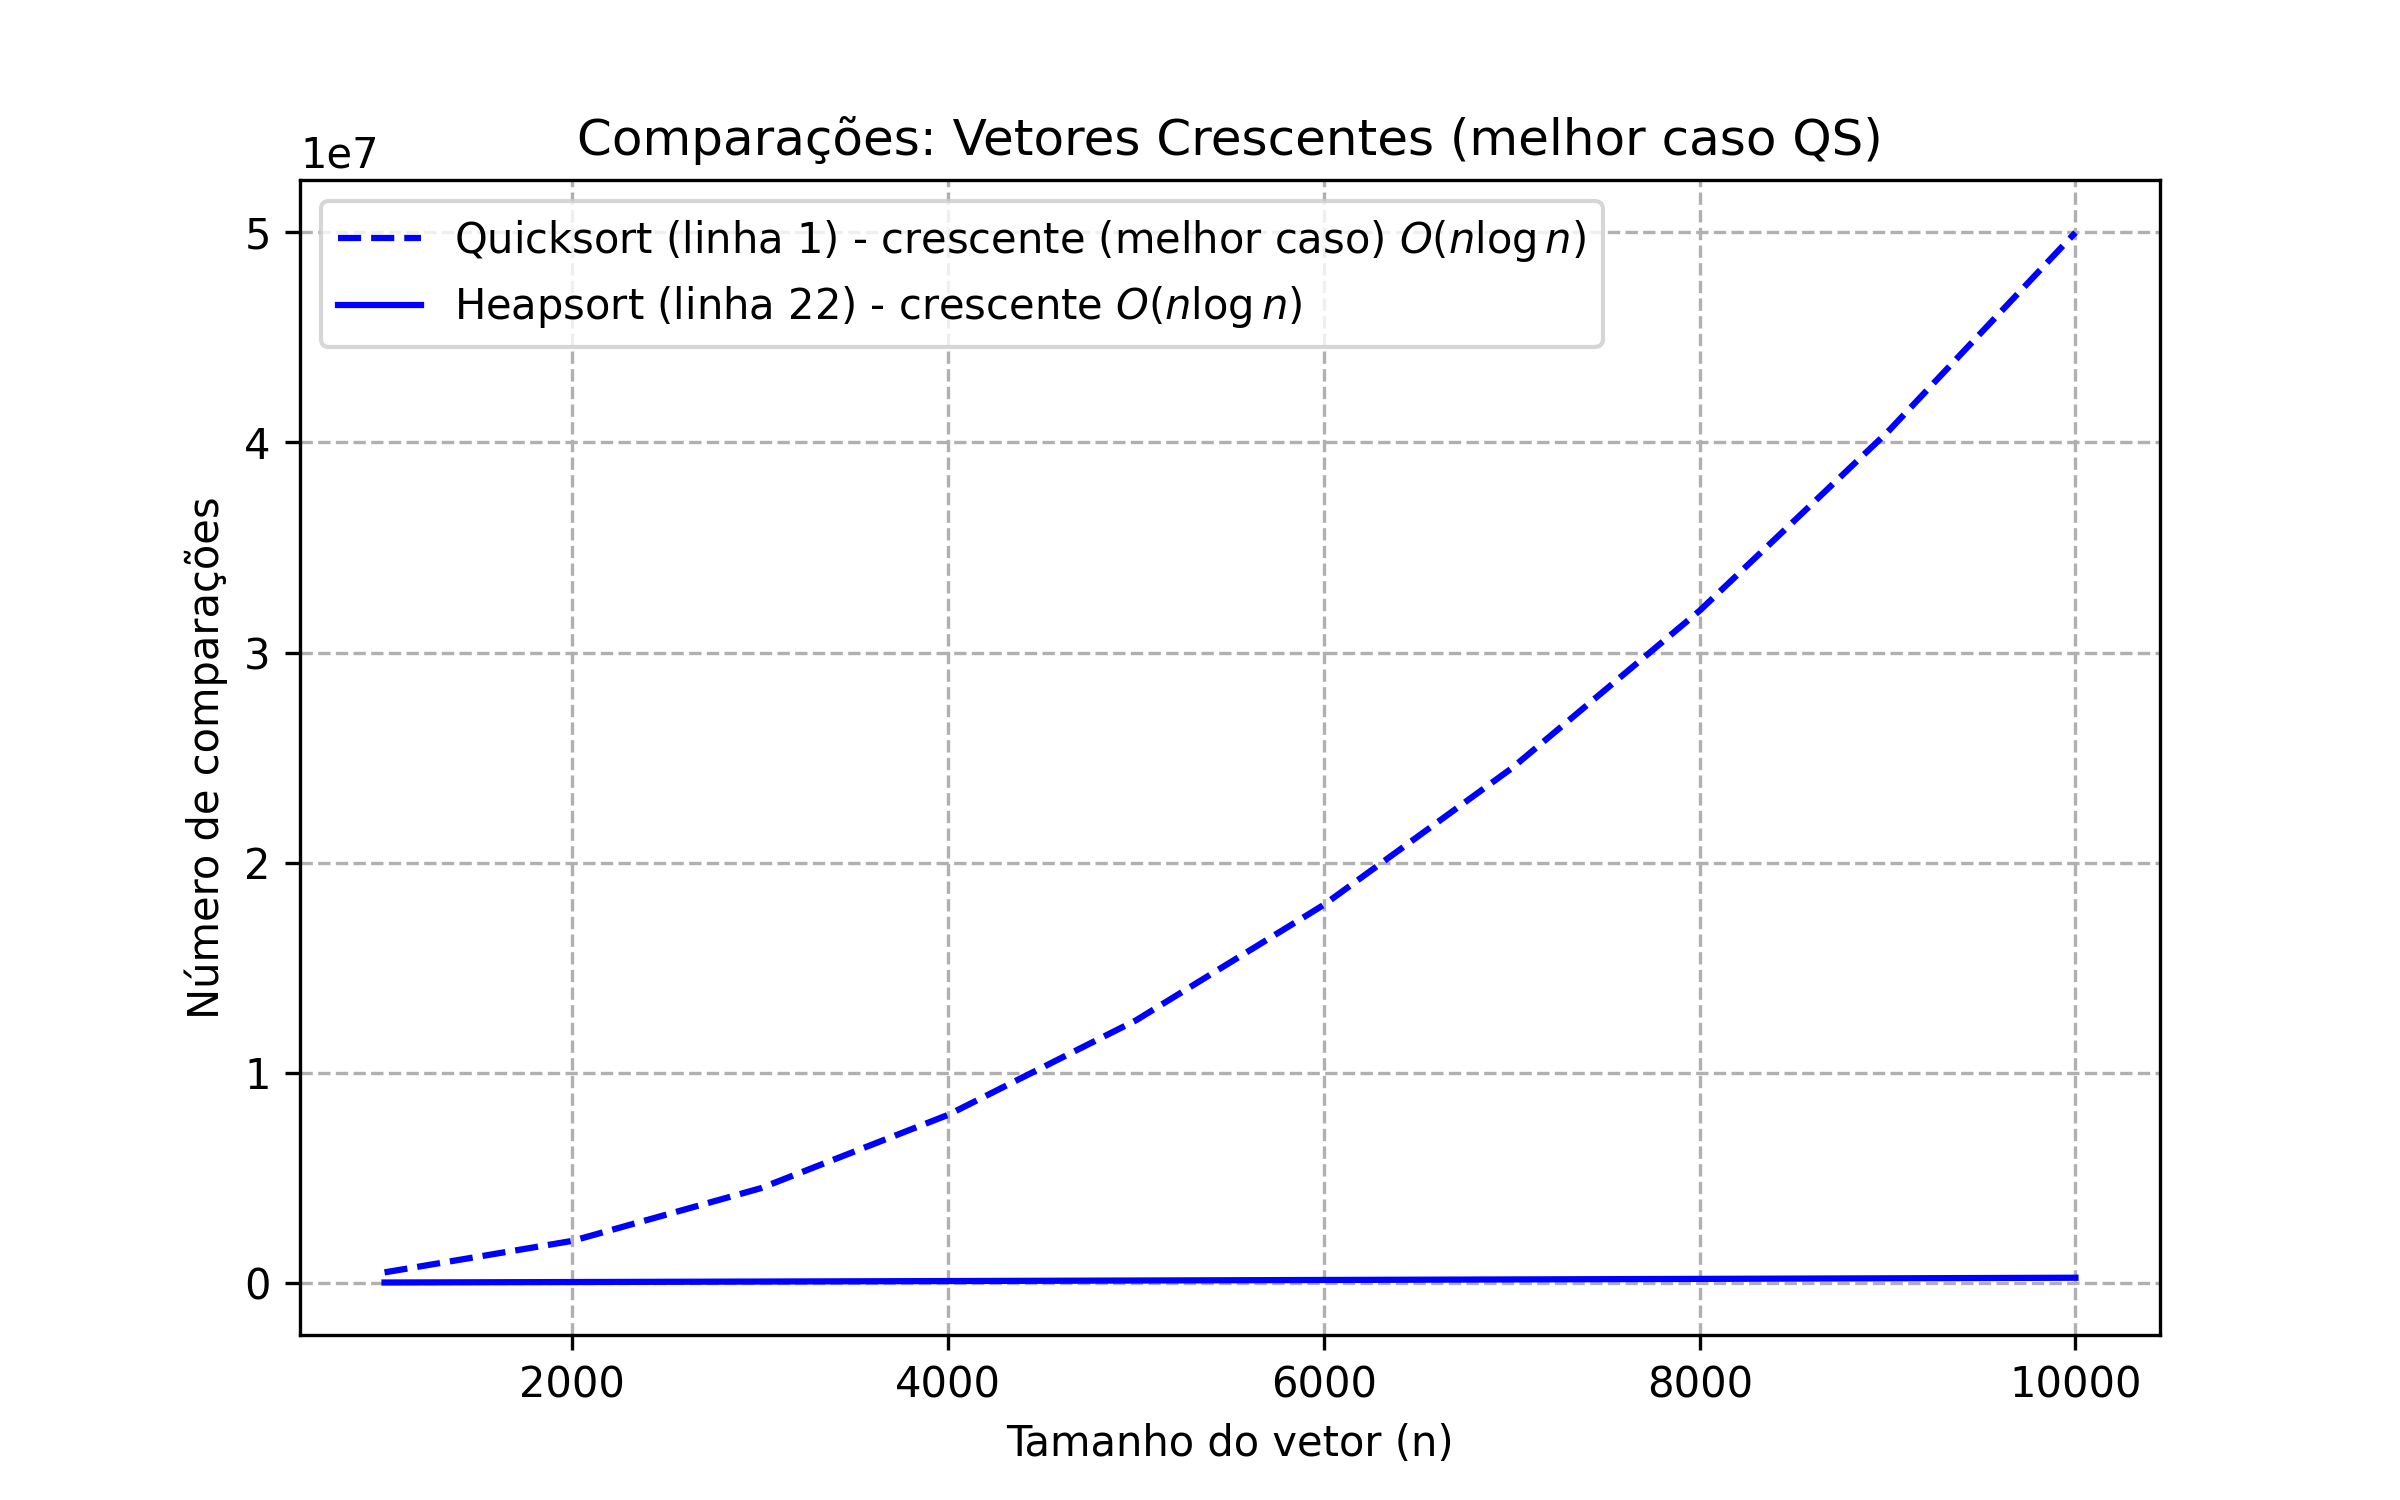
\includegraphics[width=0.8\textwidth]{../img/grafico_crescente.png}
    \caption{Número de comparações: Quicksort vs Heapsort para vetores ordenados em ordem crescente (escala linear).}
    \label{fig:crescente}
\end{figure}

Para melhor visualização das diferenças de desempenho, também foi plotado o gráfico na escala logarítmica no eixo $y$ (Figura~\ref{fig:crescente_log}):

\begin{figure}[H]
    \centering
    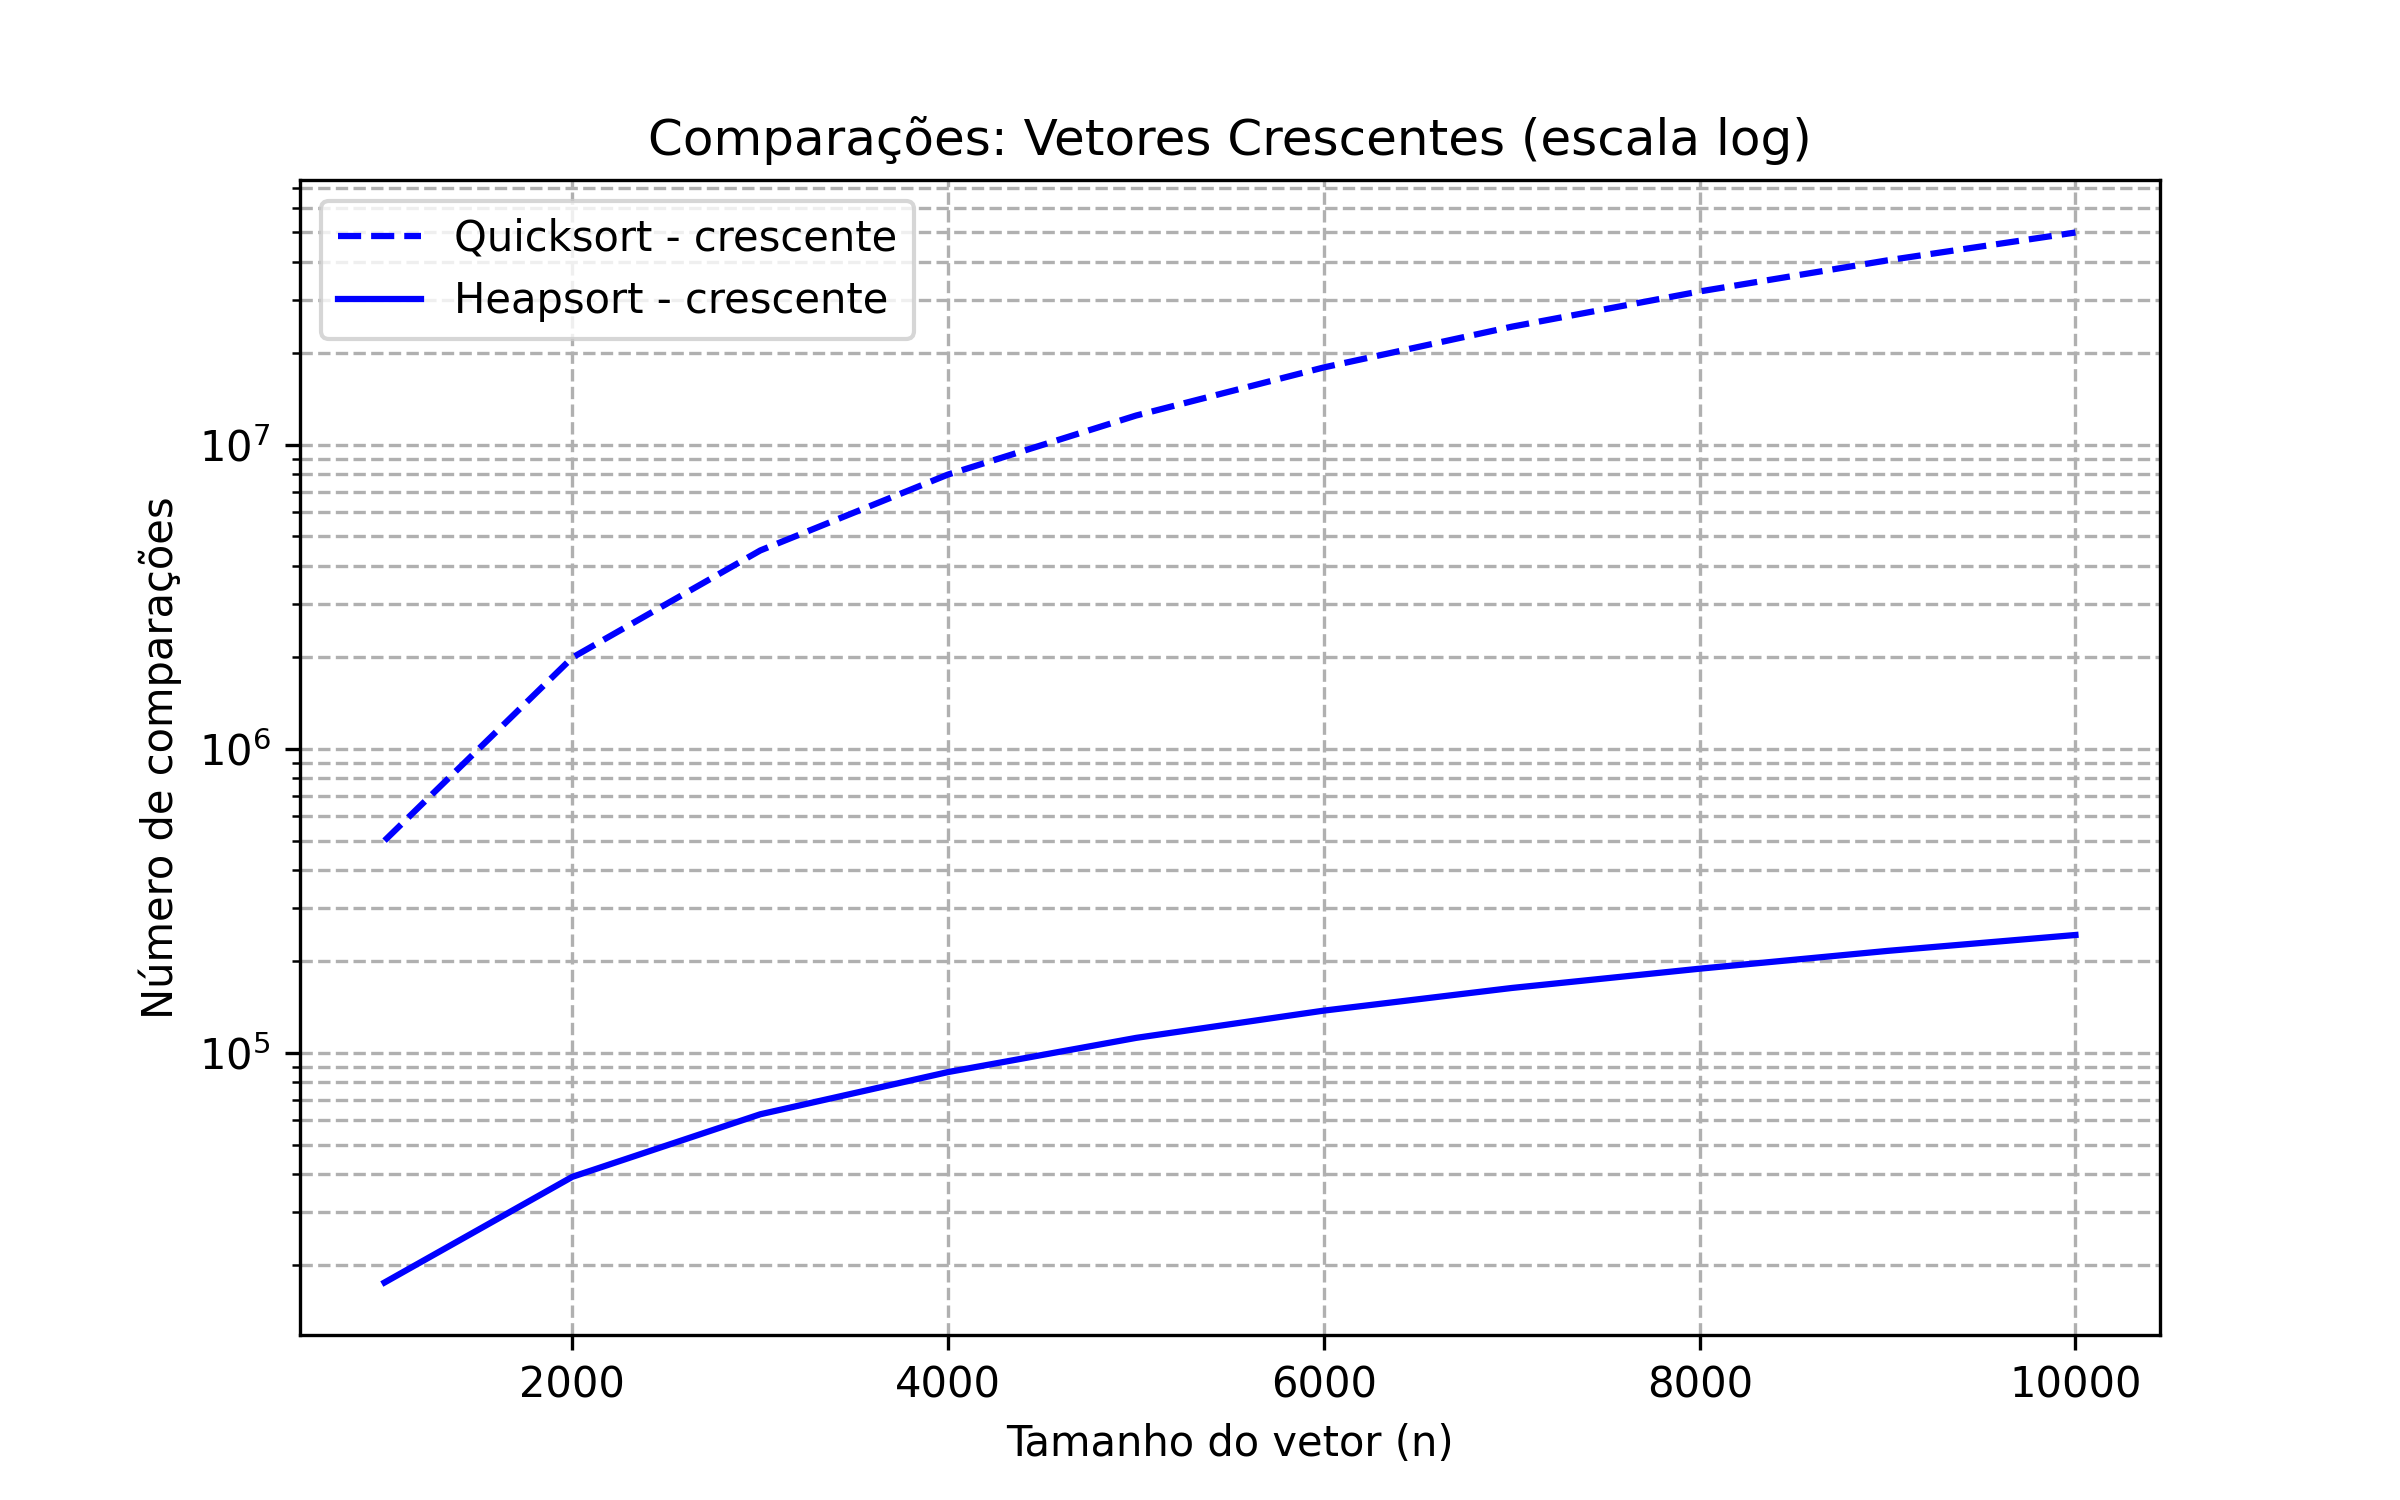
\includegraphics[width=0.8\textwidth]{../img/grafico_crescente_log.png}
    \caption{Número de comparações: Quicksort vs Heapsort para vetores ordenados em ordem crescente (escala logarítmica).}
    \label{fig:crescente_log}
\end{figure}

Apesar de ambos apresentarem complexidade assintótica $O(n \log n)$ tanto no melhor caso (vetores ordenados) quanto no caso médio (vetores aleatórios), os gráficos mostram que o Quicksort realiza um número significativamente menor de comparações do que o Heapsort nessas situações. Isso ocorre porque, além do termo dominante, os fatores constantes e termos independentes diferem: no Quicksort, o termo constante $cn$ é menor, enquanto no Heapsort há um termo linear adicional $O(n)$ devido à construção e manutenção do heap. Assim, na prática, o Quicksort tende a ser mais eficiente em número de comparações, mesmo com a mesma ordem de complexidade teórica.

\subsubsection{Resultados para Vetores Ordenados em Ordem Decrescente (Pior Caso)}

Foram gerados vetores ordenados em ordem decrescente, variando de 1000 a 10.000 elementos. Cada vetor foi ordenado utilizando Quicksort e Heapsort, e o número de comparações foi registrado.

O gráfico (Figura~\ref{fig:decrescente}) mostra o número de comparações realizadas por cada algoritmo para vetores ordenados em ordem decrescente:

\begin{figure}[H]
    \centering
    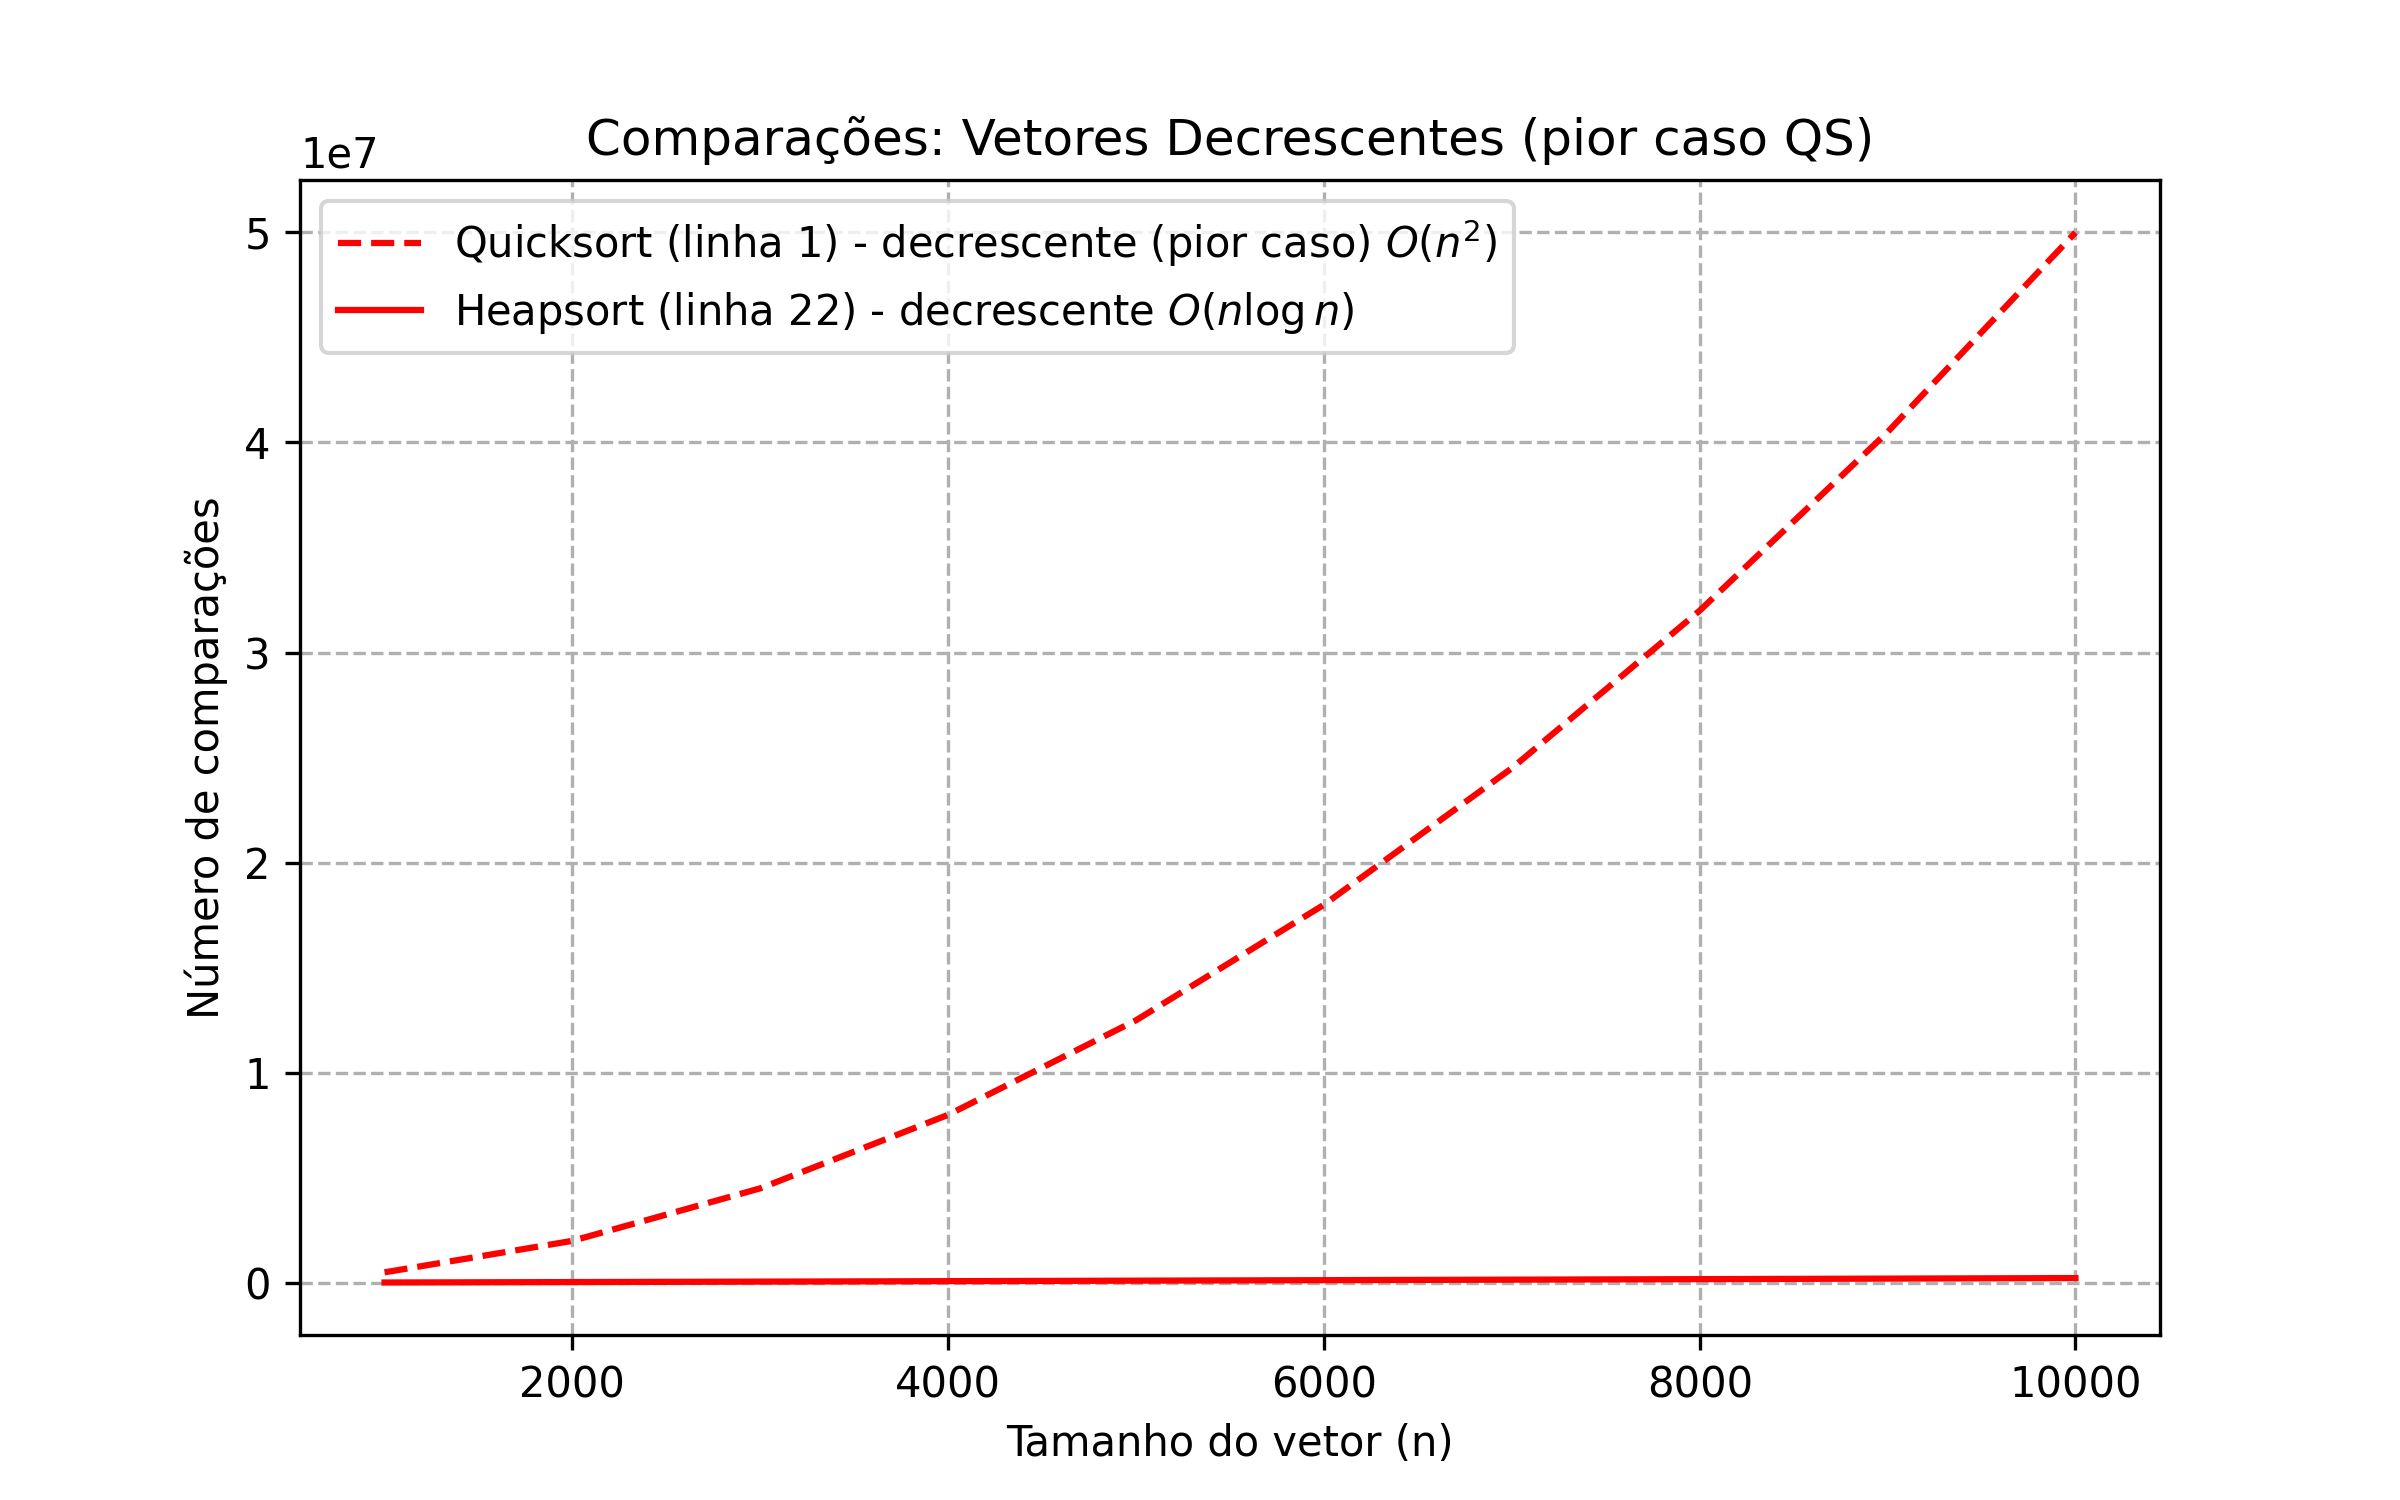
\includegraphics[width=0.8\textwidth]{../img/grafico_decrescente.png}
    \caption{Número de comparações: Quicksort vs Heapsort para vetores ordenados em ordem decrescente (escala linear).}
    \label{fig:decrescente}
\end{figure}

Para melhor visualização das diferenças de desempenho, também foi plotado o gráfico na escala logarítmica no eixo $y$ (Figura~\ref{fig:decrescente_log}):

\begin{figure}[H]
    \centering
    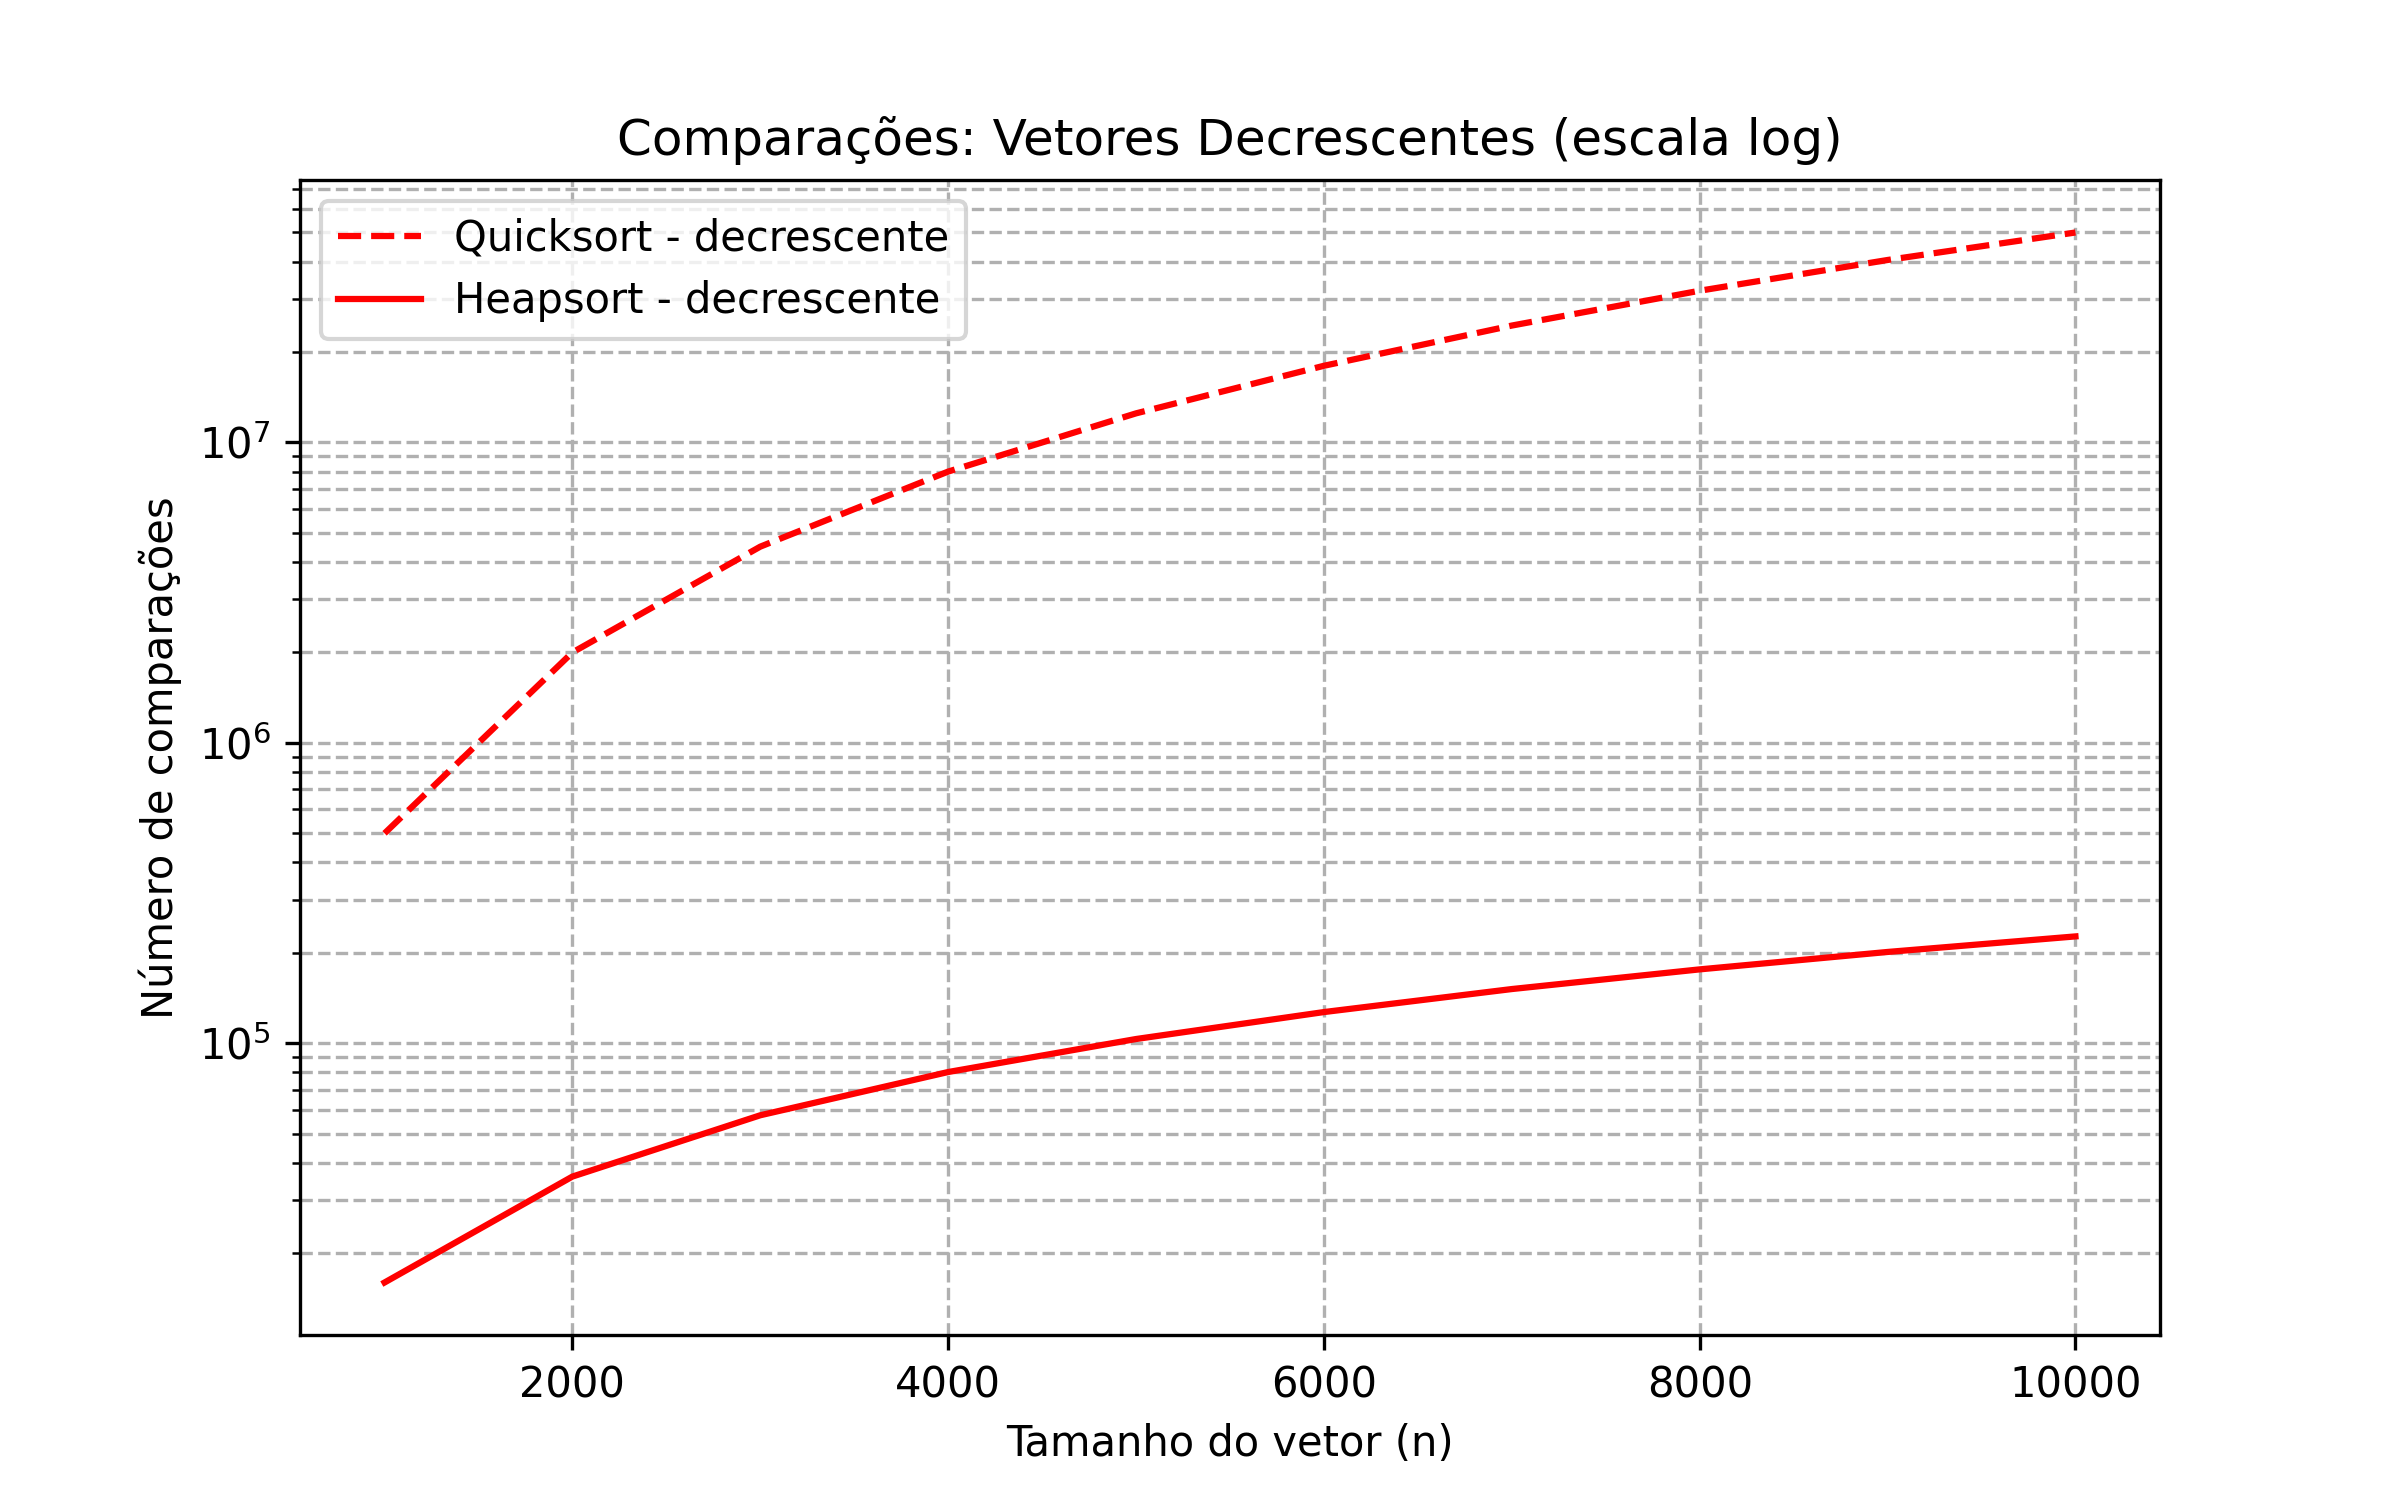
\includegraphics[width=0.8\textwidth]{../img/grafico_decrescente_log.png}
    \caption{Número de comparações: Quicksort vs Heapsort para vetores ordenados em ordem decrescente (escala logarítmica).}
    \label{fig:decrescente_log}
\end{figure}

No pior caso, que ocorre para o Quicksort quando o vetor está ordenado em ordem decrescente (ou crescente, com pivô fixo no início), o número de comparações cresce quadraticamente, resultando em complexidade $O(n^2)$. Isso é claramente observado nos gráficos, onde o Quicksort apresenta um crescimento muito mais acentuado no número de comparações em relação ao Heapsort. O Heapsort, por sua vez, mantém sua complexidade $O(n \log n)$ mesmo no pior caso, mostrando-se mais robusto e estável independentemente da ordem inicial dos dados.

\subsubsection{Resultados para Vetores Aleatórios (Caso Médio)}

Foram gerados vetores com elementos aleatórios, variando de 1000 a 10.000 elementos. Cada vetor foi ordenado utilizando Quicksort e Heapsort, e o número de comparações foi registrado.

O gráfico (Figura~\ref{fig:aleatorio}) mostra o número de comparações realizadas por cada algoritmo para vetores aleatórios:

\begin{figure}[H]
    \centering
    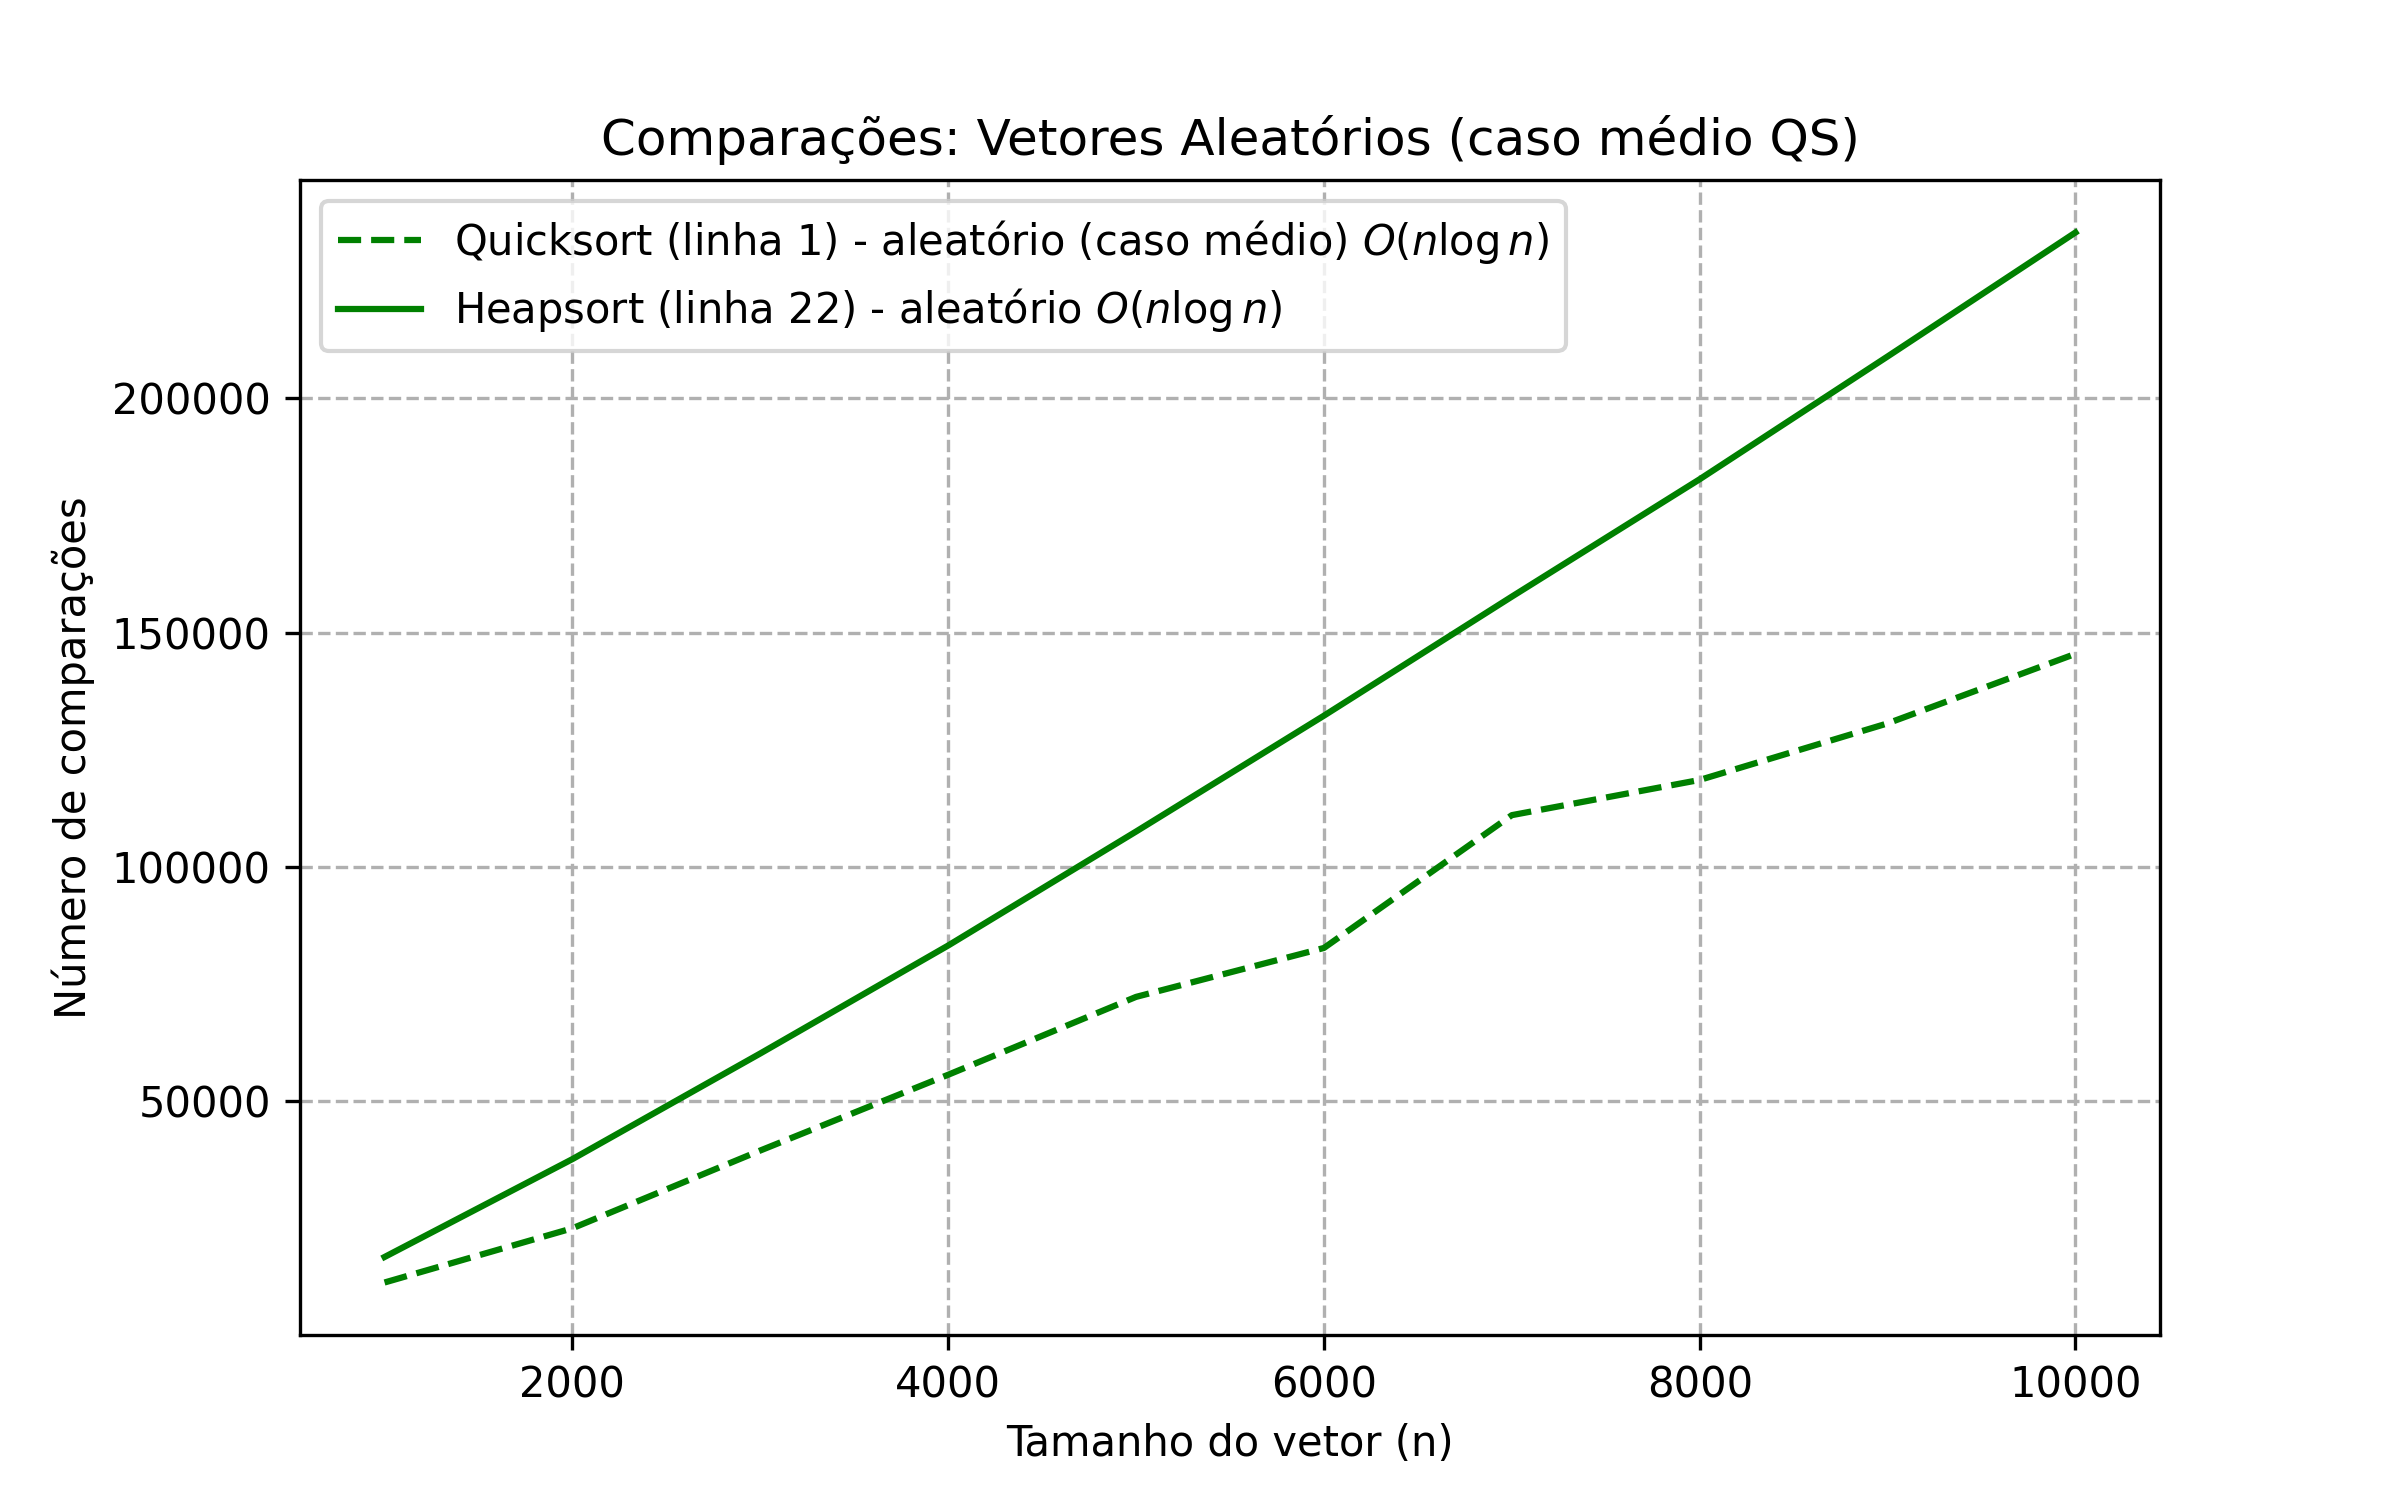
\includegraphics[width=0.8\textwidth]{../img/grafico_aleatorio.png}
    \caption{Número de comparações: Quicksort vs Heapsort para vetores aleatórios (escala linear).}
    \label{fig:aleatorio}
\end{figure}

Para melhor visualização das diferenças de desempenho, também foi plotado o gráfico na escala logarítmica no eixo $y$ (Figura~\ref{fig:aleatorio_log}):

\begin{figure}[h!]
    \centering
    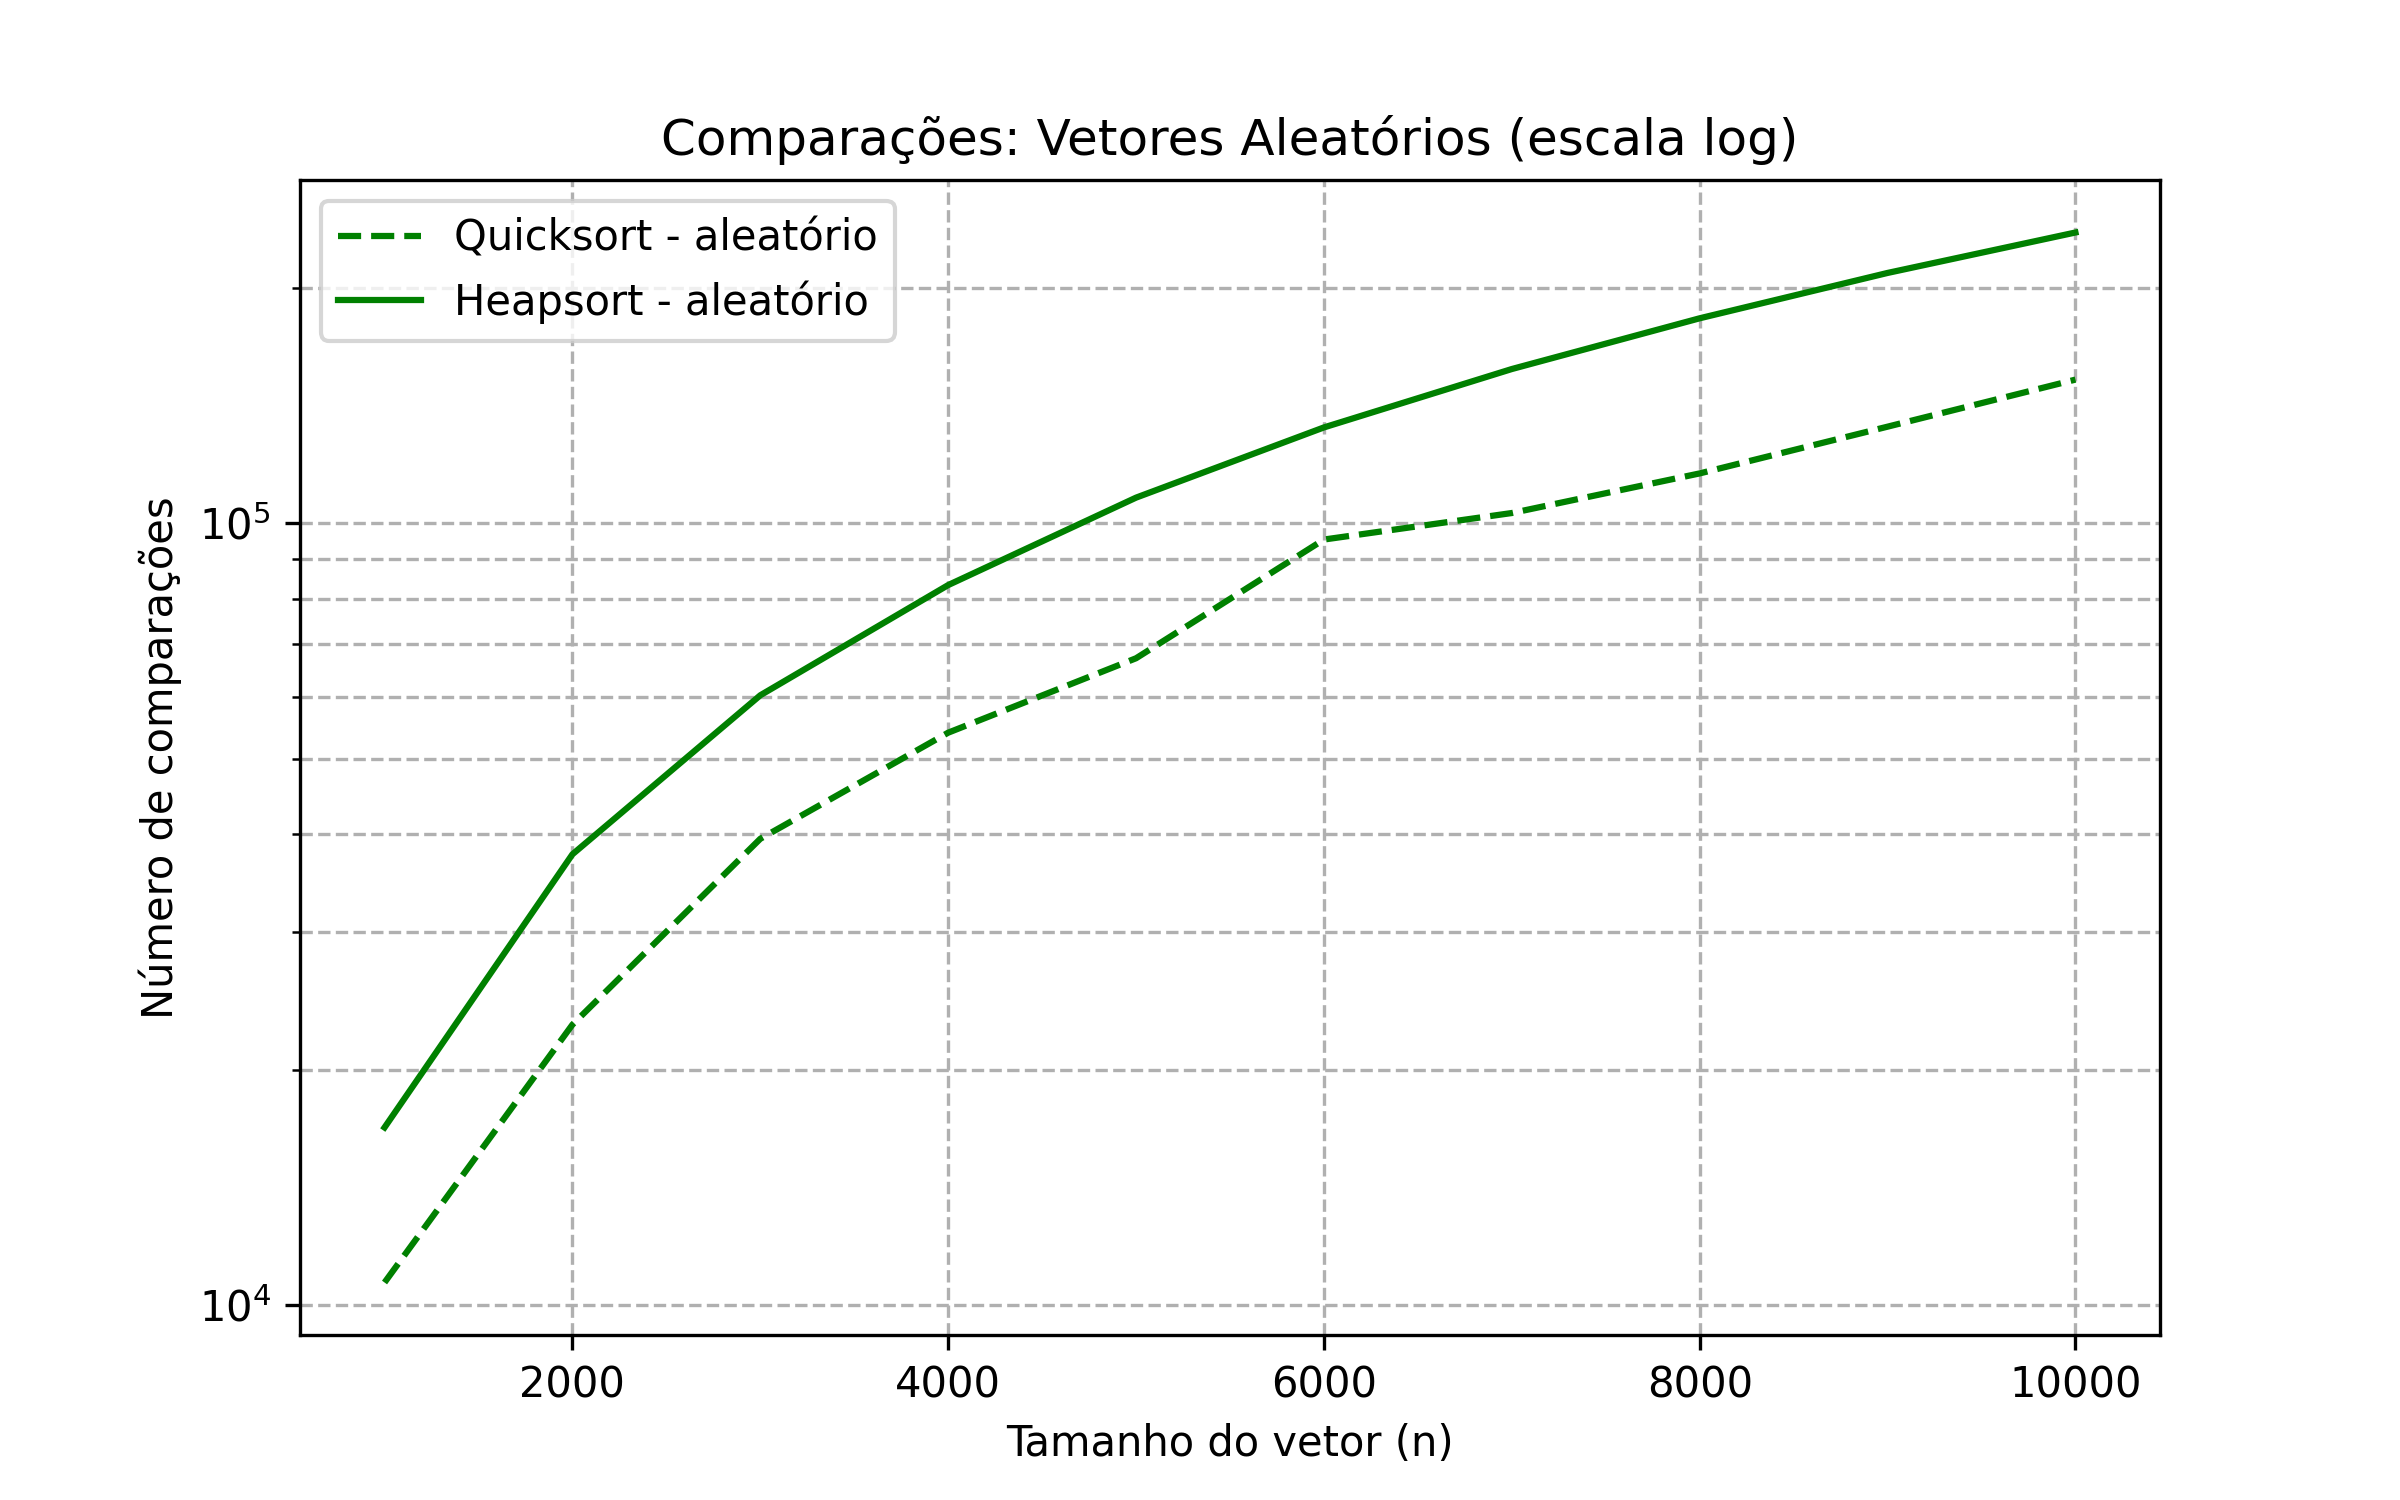
\includegraphics[width=0.8\textwidth]{../img/grafico_aleatorio_log.png}
    \caption{Número de comparações: Quicksort vs Heapsort para vetores aleatórios (escala logarítmica).}
    \label{fig:aleatorio_log}
\end{figure}

No caso dos vetores aleatórios, ambos os algoritmos mantêm a complexidade $O(n \log n)$, mas o Quicksort ainda realiza menos comparações, pois tende a dividir o vetor de forma mais equilibrada. O Heapsort, apesar de estável, apresenta um custo adicional nas operações de construção e manutenção do heap, resultando em um número de comparações um pouco maior na prática, mesmo mantendo a mesma ordem de complexidade.

Para vetores ordenados em ordem decrescente, o comportamento é semelhante ao do caso crescente: o Quicksort sofre com divisões desbalanceadas, resultando em complexidade quadrática $O(n^2)$ e um número muito elevado de comparações. O Heapsort, por outro lado, mantém desempenho estável e próximo de $O(n \log n)$, independentemente da ordem inicial dos dados. Isso evidencia que o Heapsort é mais robusto frente a diferentes tipos de entrada, enquanto o Quicksort é mais sensível à escolha do pivô e à ordem dos dados.

\section{Conclusão}

A análise dos resultados experimentais, ilustrados nos gráficos consolidados das Figuras~\ref{fig:consolidado} e~\ref{fig:consolidado_log}, evidencia diferenças marcantes entre Quicksort e Heapsort conforme o tipo de entrada.

O gráfico da Figura~\ref{fig:consolidado} apresenta todos os cenários juntos, permitindo comparar o comportamento dos algoritmos em diferentes tipos de entrada:

\begin{figure}[H]
    \centering
    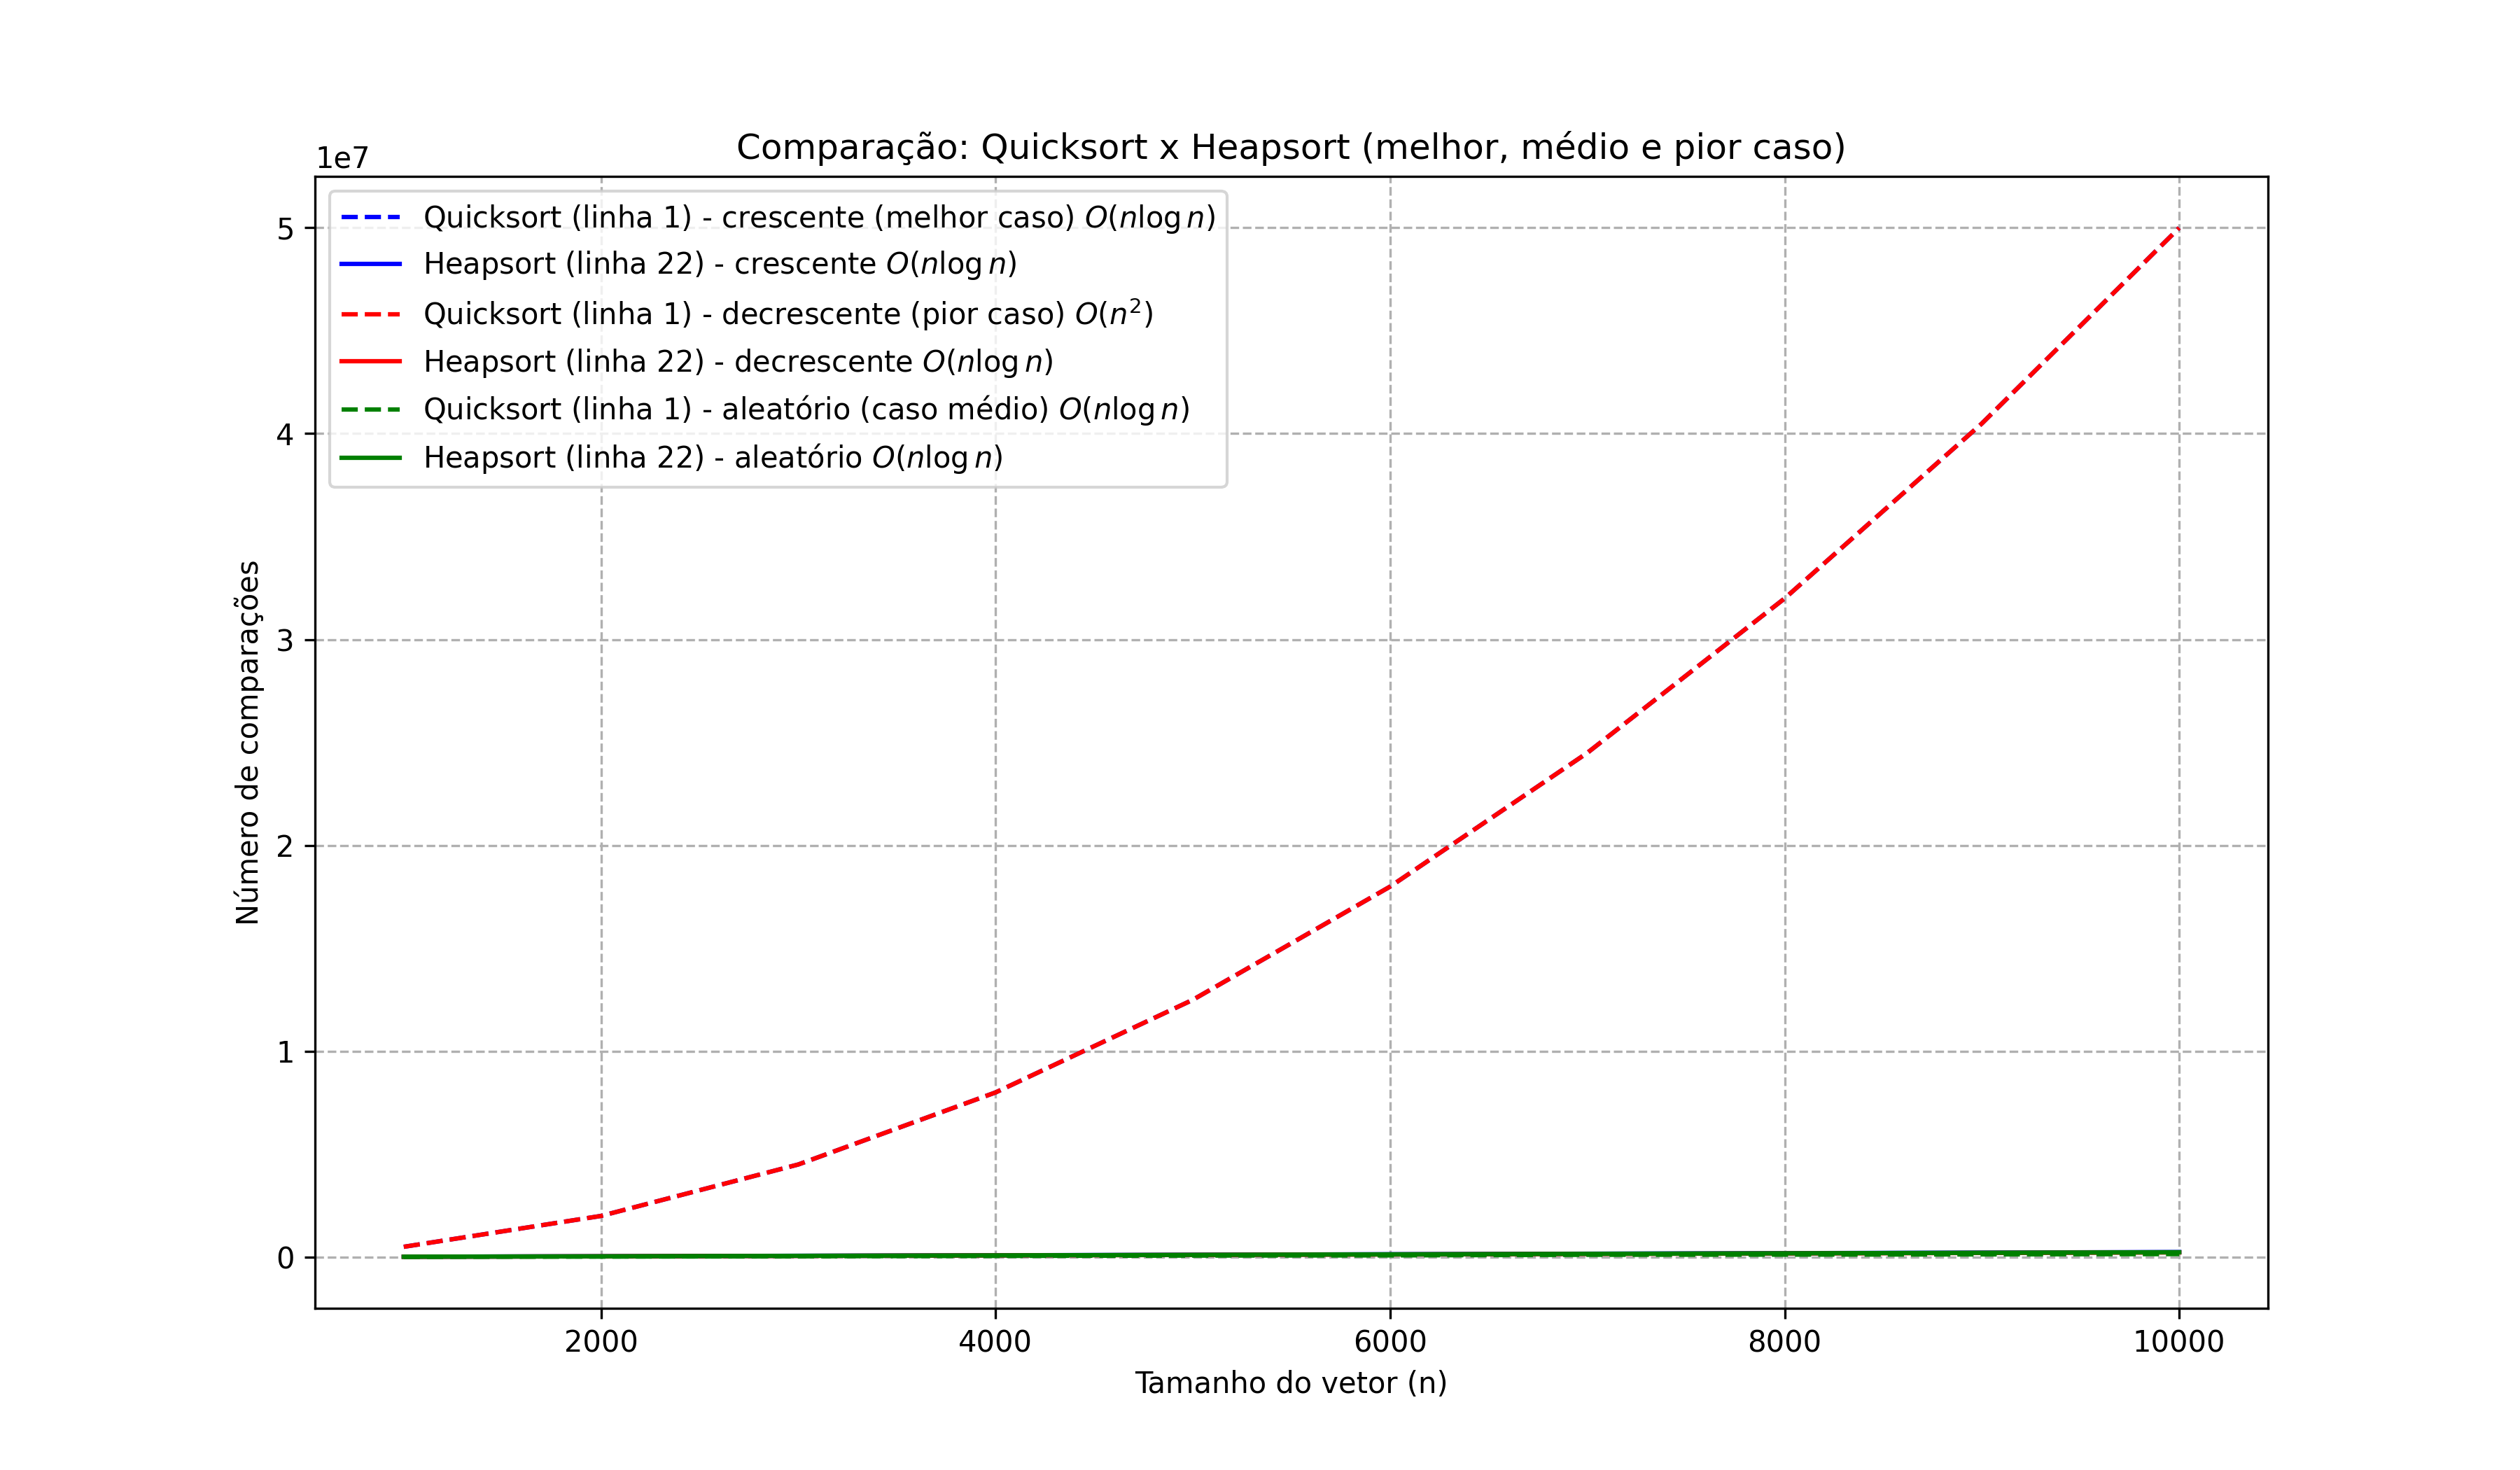
\includegraphics[width=0.9\textwidth]{../img/grafico_comparacoes.png}
    \caption{Número de comparações: Quicksort vs Heapsort para diferentes tipos de entrada (escala linear).}
    \label{fig:consolidado}
\end{figure}

Para análise em escala logarítmica, foi gerado também o gráfico da Figura~\ref{fig:consolidado_log}:

\begin{figure}[h!]
    \centering
    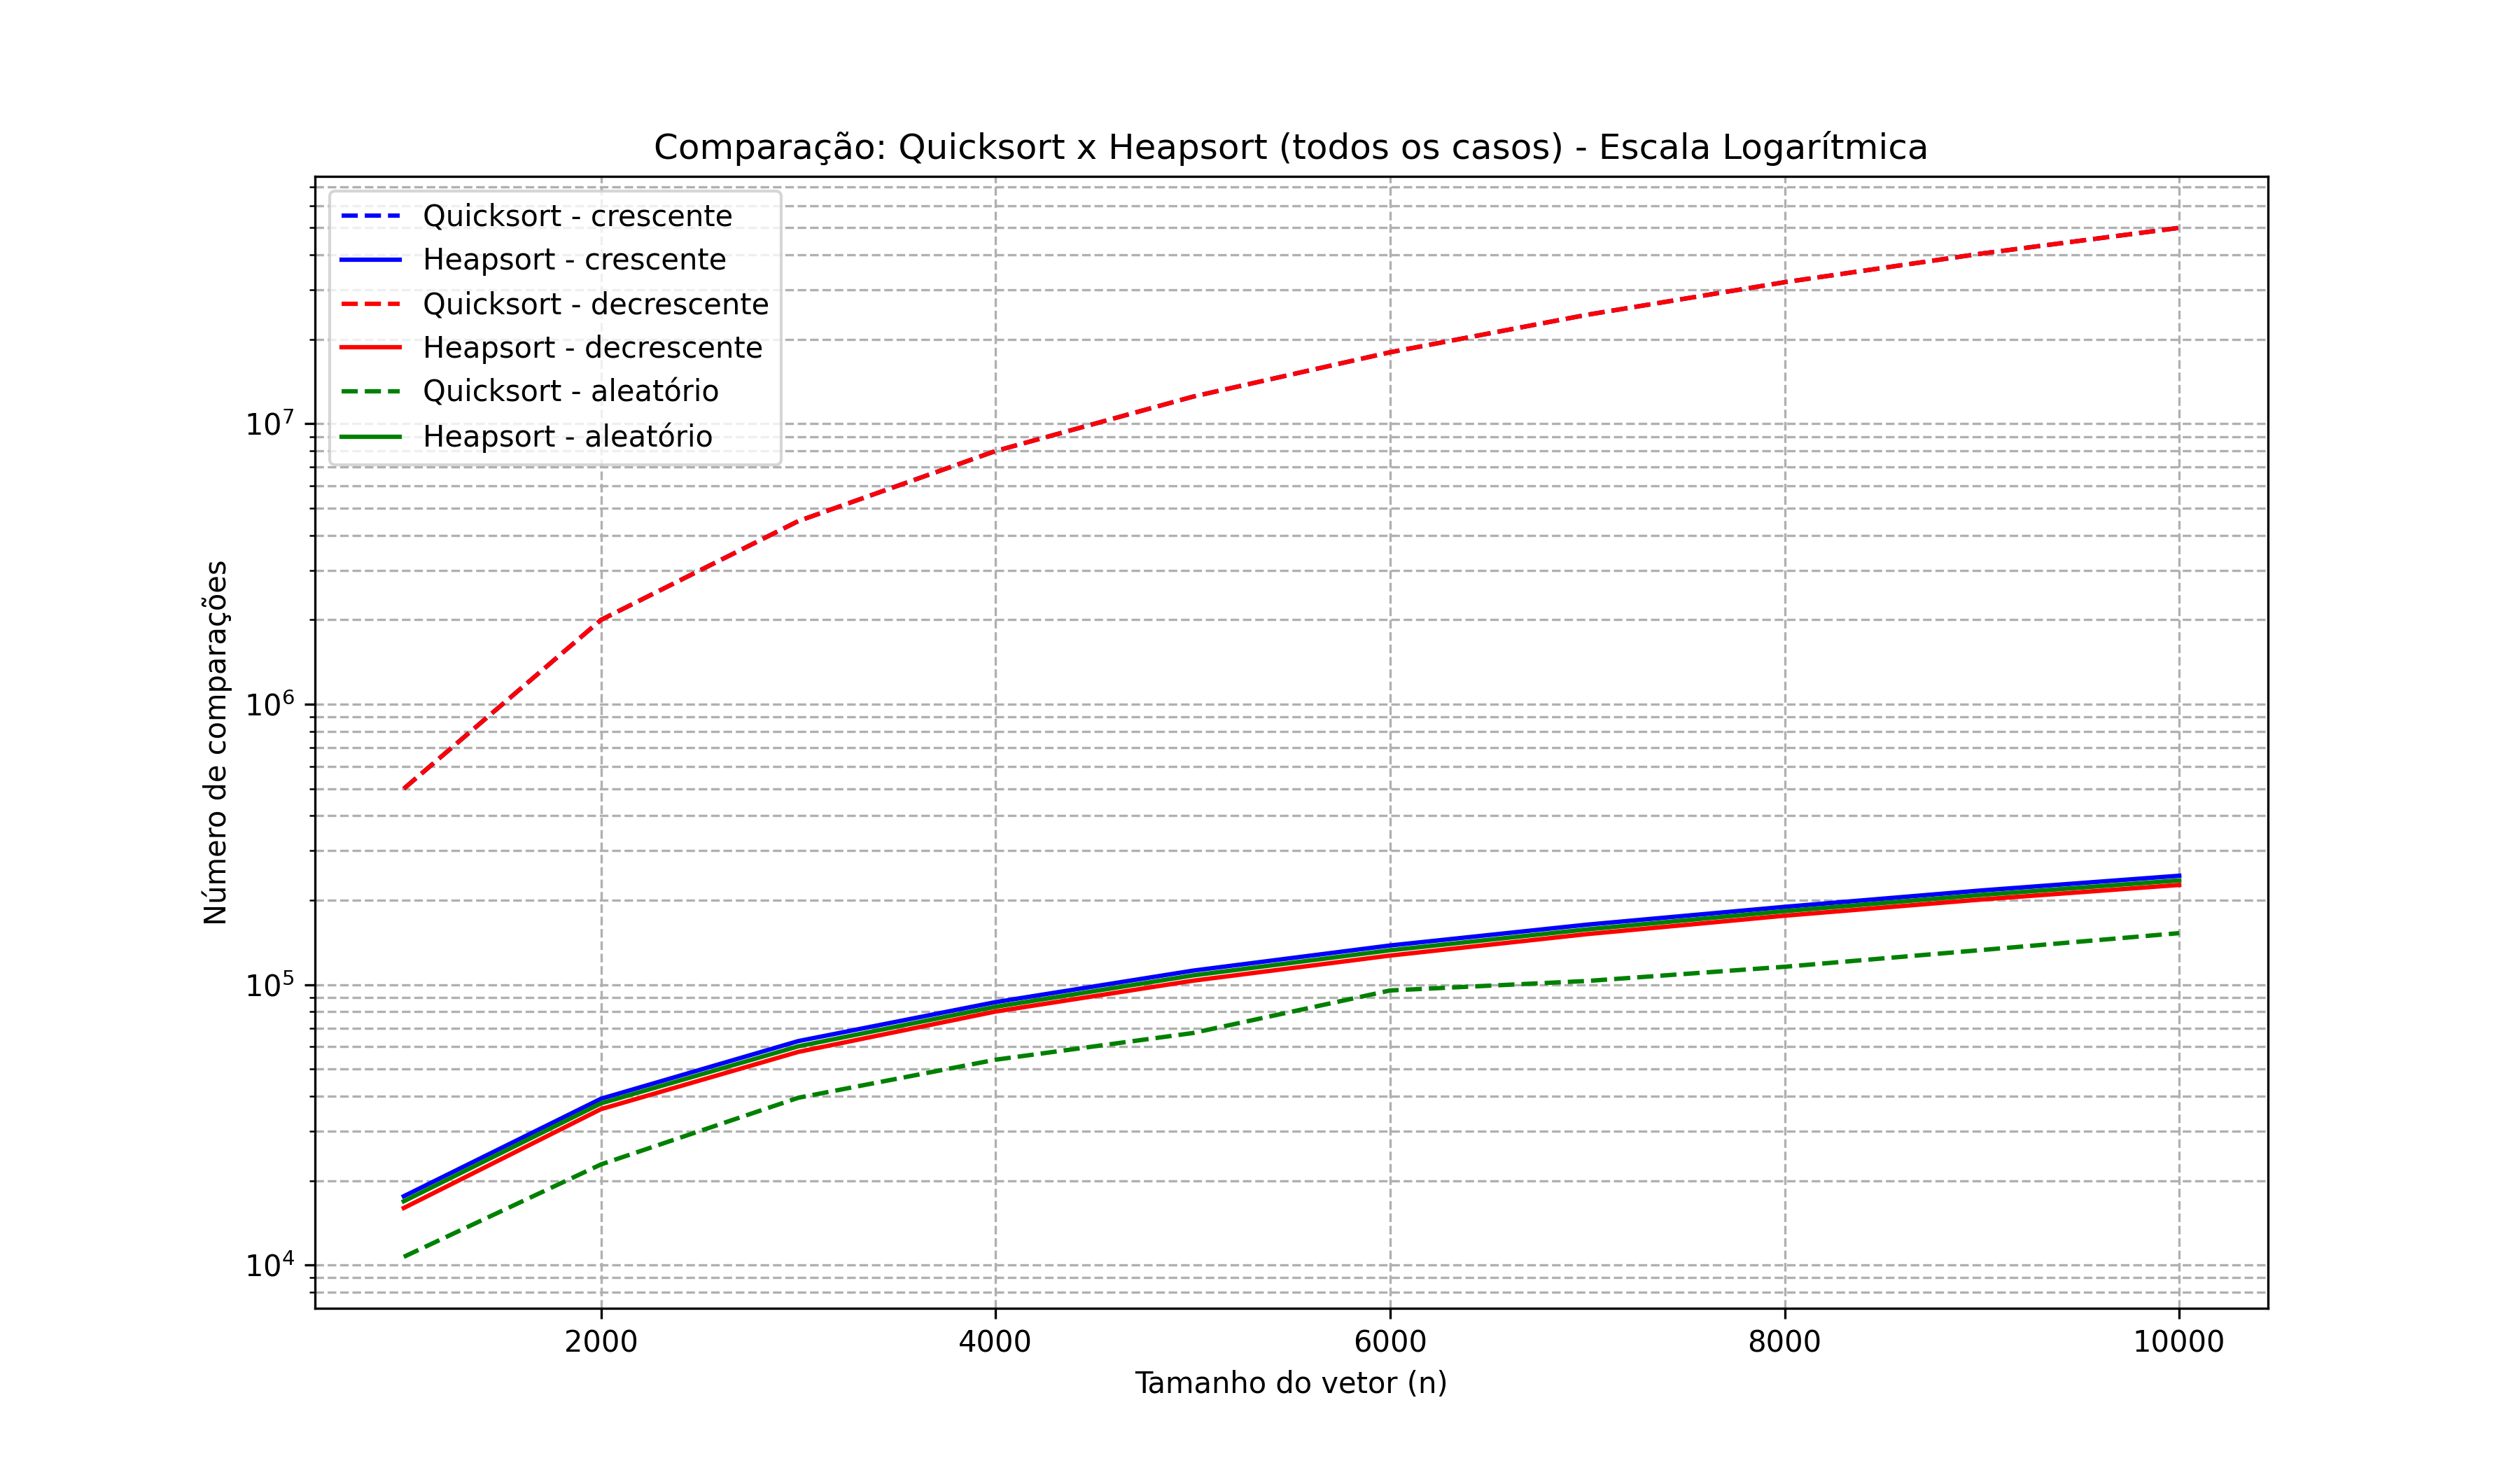
\includegraphics[width=0.9\textwidth]{../img/grafico_comparacoes_log.png}
    \caption{Número de comparações: Quicksort vs Heapsort para diferentes tipos de entrada (escala logarítmica).}
    \label{fig:consolidado_log}
\end{figure}

Para vetores ordenados (crescente), o Quicksort apresenta desempenho superior, realizando um número significativamente menor de comparações do que o Heapsort, mesmo ambos tendo complexidade $O(n \log n)$. Isso se deve ao menor fator constante do Quicksort, já que o Heapsort possui um termo linear adicional devido à construção do heap.

No caso de vetores aleatórios, ambos os algoritmos mantêm a complexidade $O(n \log n)$, mas o Quicksort ainda realiza menos comparações, pois tende a dividir o vetor de forma mais equilibrada. O Heapsort, apesar de estável, apresenta um custo adicional nas operações de construção e manutenção do heap, resultando em um número de comparações um pouco maior na prática, mesmo mantendo a mesma ordem de complexidade.

Para vetores ordenados em ordem decrescente, o Quicksort sofre seu pior caso, com crescimento quadrático $O(n^2)$ no número de comparações, tornando-se muito menos eficiente que o Heapsort, que mantém sua robustez e estabilidade com $O(n \log n)$.

Portanto, os experimentos mostram que o Quicksort é mais eficiente em entradas aleatórias ou ordenadas, mas pode ser muito penalizado em casos desfavoráveis. O Heapsort, por sua vez, é mais estável e previsível, sendo indicado quando se deseja garantir desempenho consistente independentemente da ordem inicial dos dados.

\end{document}